\documentclass[11pt,a4paper]{article}
\usepackage[utf8]{inputenc}
\usepackage[T1]{fontenc}
\usepackage{amsmath,amssymb}
\usepackage{booktabs,graphicx,caption,siunitx}
\usepackage[numbers,sort&compress]{natbib}
\usepackage[margin=2.5cm]{geometry}
\usepackage{hyperref}
\newcommand{\Fone}{F_1}
\DeclareMathOperator*{\argmax}{arg\,max}

\title{Label-Verified Pseudo-Alignment and Joint Registration by Recognition for Weakly Supervised Reading of Identity-Card Fields on Hand-Held Photographs}
\author{Draft --- authors and affiliations to be added}
\date{Working draft of 28 November 2026 --- not submitted}

\begin{document}
\maketitle

\begin{abstract}
Reading the national identifier and the dates of an identity card photographed by hand is a recurring step of remote identity verification. Systems that segment a line into glyphs fail on imperfectly rectified photographs, and training a line recogniser normally requires transcriptions \emph{and} aligned crops. We study a CPU-only setting in which the only supervision is the line-level text that a verification database already holds. We propose (i) \emph{label-verified pseudo-alignment}, which places each training window where a bootstrap recogniser reproduces the known label, so mis-registered cards never teach noise, and (ii) \emph{joint registration by recognition}, which estimates the residual shift and scale of a card by maximising the summed CTC confidence of all fields read under one geometric hypothesis. A 1.1\,M-parameter CRNN/CTC model (4\,MB, ONNX Runtime, no GPU) trained with these ideas on 1{,}376 photographs is evaluated on 400 held-out photographs of a public dataset of \emph{fictitious} Iranian national ID cards. Against a segment-and-classify pipeline, macro $\Fone$ over three fields rises from 0.487 to 0.705 and the precision of auto-accepted values is 0.978--0.996. The CTC confidence separates correct from incorrect readings (AUC $\ge 0.99$; ECE 0.016). The data are synthetic and single-design, the split is single, and no second benchmark is used; these limits are discussed explicitly.
\end{abstract}

\noindent\textbf{Keywords:} identity document recognition; CRNN; connectionist temporal classification; weak supervision; document registration; KYC.

\section{Introduction}
Remote onboarding depends on reading identity-card fields from photographs taken with consumer devices. Two properties of the setting shape the problem. First, photographs are rectified from detected card corners that are imprecise, so text lines land at unpredictable offsets and scales. Second, production systems hold \emph{labels without geometry}: the identifier and dates are in a database, but nobody annotated where they appear in each image. Resource limits (no GPU, one or two CPU cores) exclude large transformer recognisers.

Our contributions are:
\begin{enumerate}
  \item a training protocol that needs only line-level labels, \emph{label-verified pseudo-alignment} (Section~\ref{sec:align});
  \item an inference procedure that uses the recogniser itself as the registration score and ties all fields to one hypothesis (Section~\ref{sec:joint});
  \item a confidence-gated decision policy with a measured precision/coverage trade-off (Section~\ref{sec:results});
  \item an open CPU-only implementation and a log of negative results.
\end{enumerate}
We do not claim a new network architecture: CRNN with CTC is standard~\cite{shi2017crnn,graves2006ctc}. The claim is limited to the supervision and registration scheme, evaluated on one dataset.

\section{Related work}
\paragraph{Sequence recognition.} CRNN with CTC~\cite{shi2017crnn,graves2006ctc} is the standard segmentation-free recogniser; Baek et al.~\cite{baek2019wrong} compare scene-text recognition modules, and transformer recognisers such as TrOCR~\cite{li2023trocr} improve accuracy at a much larger computational cost. We keep a small CRNN because of the CPU budget.
\paragraph{Identity documents.} The MIDV family~\cite{arlazarov2019midv500,bulatov2022midv2020} provides mobile captures of identity documents. Open engines such as Tesseract~\cite{smith2007tesseract} are the usual off-the-shelf baseline.
\paragraph{Pseudo-labelling.} Self-training on model-predicted labels~\cite{lee2013pseudo} is sensitive to wrong labels. Our alignment is \emph{verifiable} because the target string is known, which removes label noise from the placement step by construction.
\paragraph{Face detection.} YuNet~\cite{wu2023yunet} is used for orientation checks and portrait extraction.
\paragraph{Gap in this survey.} Document localisation and rectification, weakly supervised OCR and KYC liveness literature are not yet reviewed; a systematic search is required before submission.

\section{Method}
\subsection{Pipeline}
The pipeline decodes the image, detects the card by contour scoring, rectifies it to $1011\times 638$ pixels by a perspective transform, determines side, version and rotation (colour/marker classifier cross-checked by a face detector), reads the fields, validates them (checksum, calendar) and stores the images encrypted.

\subsection{Windows and hypotheses}
For a field $f$ with nominal centre $\mathbf{c}_f\in\mathbb{R}^2$ and a common anchor $\mathbf{a}$, a hypothesis $h=(s,\Delta y,\Delta x)$ defines the window centre
\begin{equation}
\mathbf{c}_f(h)=\mathbf{a}+\tfrac{1}{s}\,(\mathbf{c}_f-\mathbf{a})+(\Delta x,\Delta y),
\label{eq:centre}
\end{equation}
and the window of fixed nominal size $360\times166$ is cropped at scale $1/s$ and resized to $112\times240$. The grid has $|\mathcal{H}|=63$ hypotheses: $s\in\{0.85,1,1.2\}$, $\Delta y\in\{-90,-60,\dots,90\}$, $\Delta x\in\{-40,0,40\}$.

\subsection{Network and decoding}
Four convolution blocks (32--64--96--128 channels) keep the vertical position in the channel axis; two bidirectional GRU layers~\cite{cho2014gru} with 128 units feed a CTC head over $K=11$ symbols (digits and ``/'') plus a blank. A constant plane encoding the field is appended to the grayscale input. With $\mathbf{x}$ the window and $\mathbf{y}$ the label, training minimises
\begin{equation}
\mathcal{L}=-\log\sum_{\pi\in\mathcal{B}^{-1}(\mathbf{y})}\prod_{t=1}^{T}p_t(\pi_t\mid\mathbf{x}),
\end{equation}
where $\mathcal{B}$ removes repeats and blanks~\cite{graves2006ctc}. Optimisation uses AdamW~\cite{loshchilov2019adamw}. The reading of a window is the greedy decoding $\hat{\mathbf{y}}$ with confidence
\begin{equation}
\kappa(\mathbf{x})=\begin{cases}\dfrac{1}{|\hat{\mathbf{y}}|}\sum_{t\in E}\max_k p_t(k\mid\mathbf{x}) & \text{if }\hat{\mathbf{y}}\text{ is well formed},\\[1ex] 0 & \text{otherwise},\end{cases}
\end{equation}
where $E$ is the set of time steps that emit a character.

\subsection{Label-verified pseudo-alignment}\label{sec:align}
Stage~1 trains a bootstrap model on nominal windows only. Stage~2 searches, for each training card $i$ with label $\mathbf{y}_i$, the set
\begin{equation}
\mathcal{V}_i=\{\,h\in\mathcal{H}:\ \hat{\mathbf{y}}(\mathbf{x}_i(h))=\mathbf{y}_i\,\}
\end{equation}
and keeps the card only if $\mathcal{V}_i\neq\emptyset$, using the verified hypothesis (the nominal one if verified, otherwise the first found). Of 1{,}376 training cards, 889 are kept. Stage~3 trains the final model on windows centred at the verified hypothesis with jitter ($\pm12$ px horizontally, $\pm10$ px vertically), rotation ($\pm6^\circ$), shear, photometric noise and 5\% empty-target windows. Dates inherit the hypothesis of the identifier through Eq.~\eqref{eq:centre}.

\subsection{Joint registration by recognition}\label{sec:joint}
At inference, the hypothesis is chosen to maximise the summed confidence of all fields,
\begin{equation}
h^\star=\argmax_{h\in\mathcal{H}}\ \sum_{f\in F}\kappa\big(\mathbf{x}_f(h)\big),\qquad F=\{\text{id},\text{birth},\text{expiry}\}.
\end{equation}
The nominal hypothesis is tried first, and the search stops if every field has $\kappa\ge0.95$. A field is auto-accepted if $\kappa\ge\tau$ with $\tau=0.9$, fixed a priori, and routed to human review otherwise.

\section{Experimental protocol}
\paragraph{Data.} The public Kaggle dataset of fictitious Iranian national ID cards~\cite{kaggleiranid}: 2{,}000 hand-held photographs with labels for identifier, dates and names. The split is by image index (index mod 5 $=0$ for the 400 test photographs). No hyper-parameter was tuned on the test photographs. \textbf{Caveats:} cards and faces are synthetic, many photographs share a face, and most identifiers fail the official checksum, so the checksum was disabled in evaluation.
\paragraph{Metrics.} Over all test photographs (a rejected photograph counts as a miss), with $N$ photographs, $A$ the auto-accepted fields and $C$ the exact matches:
\begin{align}
\text{accuracy}&=\frac{|C|}{N}, & \text{precision}&=\frac{|C\cap A|}{|A|}, & \text{recall}&=\frac{|C\cap A|}{N},\\
\Fone&=\frac{2\,\text{precision}\cdot\text{recall}}{\text{precision}+\text{recall}}.
\end{align}
Confidence intervals are 95\% percentile bootstrap intervals over photographs with 2{,}000 draws~\cite{efron1993bootstrap}. Paired differences use the exact McNemar test~\cite{mcnemar1947} on exact matches and a paired bootstrap of $\Delta\Fone$. Calibration is summarised by the expected calibration error~\cite{guo2017calibration},
\begin{equation}
\text{ECE}=\sum_{b=1}^{B}\frac{n_b}{n}\,\bigl|\text{acc}(b)-\text{conf}(b)\bigr|,\quad B=10 .
\end{equation}
\paragraph{Baselines.} (a) Tesseract~\cite{smith2007tesseract} on the nominal window; (b) EasyOCR (generic Persian/Arabic-script model, nominal window, no fine-tuning, same acceptance rule); (c) a segment-and-classify pipeline (connected components, HOG features, $k$-NN trained on the same real glyphs); (d) the proposed method.

\section{Results}\label{sec:results}
\subsection{Main comparison}
Table~\ref{tab:main} gives $\Fone$ on the 400 test photographs through the full pipeline, and Table~\ref{tab:pr} gives accuracy, precision and recall. Fig.~\ref{fig:f1} shows the same $\Fone$ values graphically.
\begin{table}[t]
\centering\small
\caption{$\Fone$ [95\% bootstrap CI], 400 test photographs, full pipeline, checksum disabled.}\label{tab:main}
\begin{tabular}{lccc}
\toprule
Method & National id & Birth date & Expiry date\\
\midrule
Tesseract & 0.135 [0.101, 0.172] & 0.273 [0.222, 0.327] & 0.198 [0.149, 0.245] \\
EasyOCR & 0.020 [0.005, 0.039] & 0.000 [0.000, 0.000] & 0.000 [0.000, 0.000] \\
Glyph + k-NN & 0.468 [0.417, 0.516] & 0.498 [0.442, 0.551] & 0.494 [0.440, 0.545] \\
Proposed & 0.723 [0.682, 0.760] & 0.704 [0.660, 0.744] & 0.687 [0.641, 0.728] \\
\bottomrule
\end{tabular}

\end{table}
\begin{table}[t]
\centering\small
\caption{Accuracy / precision / recall of auto-accepted values (same runs as Table~\ref{tab:main}).}\label{tab:pr}
\setlength{\tabcolsep}{4pt}
\begin{tabular}{lccccccccc}
\toprule
 & \multicolumn{3}{c}{National id} & \multicolumn{3}{c}{Birth date} & \multicolumn{3}{c}{Expiry date}\\
\cmidrule(lr){2-4}\cmidrule(lr){5-7}\cmidrule(lr){8-10}
Method & Acc & Prec & Rec & Acc & Prec & Rec & Acc & Prec & Rec\\
\midrule
Tesseract & 0.120 & 0.154 & 0.120 & 0.172 & 0.657 & 0.172 & 0.120 & 0.565 & 0.120 \\
EasyOCR & 0.020 & 0.444 & 0.010 & 0.000 & 0.000 & 0.000 & 0.000 & 0.000 & 0.000 \\
Glyph + k-NN & 0.417 & 0.532 & 0.417 & 0.343 & 0.913 & 0.343 & 0.335 & 0.944 & 0.335 \\
Proposed & 0.568 & 0.996 & 0.568 & 0.550 & 0.978 & 0.550 & 0.530 & 0.986 & 0.527 \\
\bottomrule
\end{tabular}

\end{table}
\begin{figure}[t]
\centering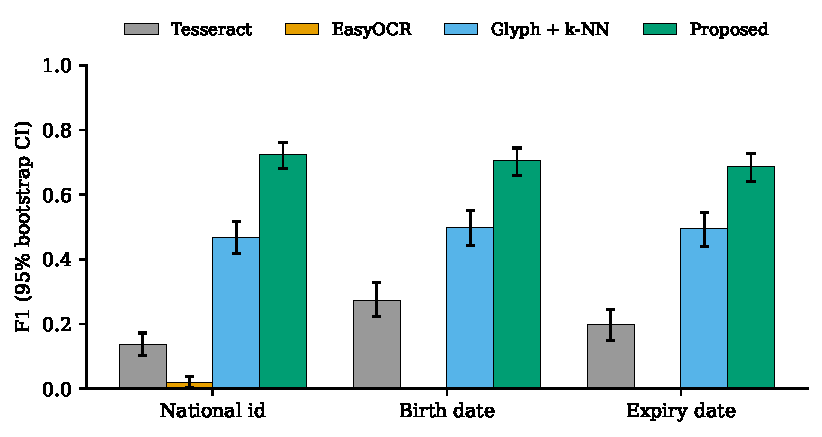
\includegraphics[width=0.85\textwidth]{figures/f1_comparison.pdf}
\caption{$\Fone$ with 95\% bootstrap intervals for the four systems.}\label{fig:f1}
\end{figure}
Paired exact-match tests between the proposed method and the segment-and-classify baseline give 60, 83 and 78 photographs read only by the proposed method (identifier, birth, expiry) against none in the other direction (McNemar $p=1.7\times10^{-18}$, $2.1\times10^{-25}$, $6.6\times10^{-24}$); the paired bootstrap $\Delta\Fone$ intervals are $[+0.22,+0.29]$, $[+0.16,+0.25]$, $[+0.15,+0.23]$. The off-the-shelf engines are near zero: they were not adapted to the card layout, and EasyOCR in particular reads the fixed window without any registration, so these rows quantify an unadapted baseline and not the limit of those engines.

\subsection{Search and alignment ablation}
Table~\ref{tab:abl} and Fig.~\ref{fig:abl} use the 325 test cards that reach the OCR stage ($\tau=0.9$). Joint registration mainly repairs the date fields, which independent per-field search confuses with the neighbouring date line (birth-date precision $0.81\to0.98$). Three seeds of the final training stage give macro $\Fone$ of $0.780\pm0.005$ (mean $\pm$ sample standard deviation, $n=3$); removing pseudo-alignment (one run) lowers it to 0.748. The bootstrap and alignment stages were not re-seeded, so this spread understates the full training variance.
\begin{table}[t]
\centering\small
\caption{Search and alignment ablation, 325 cards, $\tau=0.9$. ``Joint'' is the reported run.}\label{tab:abl}
\begin{tabular}{lccccc}
\toprule
Variant & id $F_1$ & birth $F_1$ & expiry $F_1$ & macro $F_1$ & macro prec.\\
\midrule
Nominal window & 0.708 & 0.708 & 0.671 & 0.695 & 0.988 \\
Per-field search & 0.797 & 0.656 & 0.784 & 0.745 & 0.929 \\
No pseudo-alignment & 0.764 & 0.733 & 0.746 & 0.748 & 0.987 \\
Joint (proposed) & 0.788 & 0.777 & 0.765 & 0.777 & 0.987 \\
\bottomrule
\end{tabular}

\end{table}
\begin{figure}[t]
\centering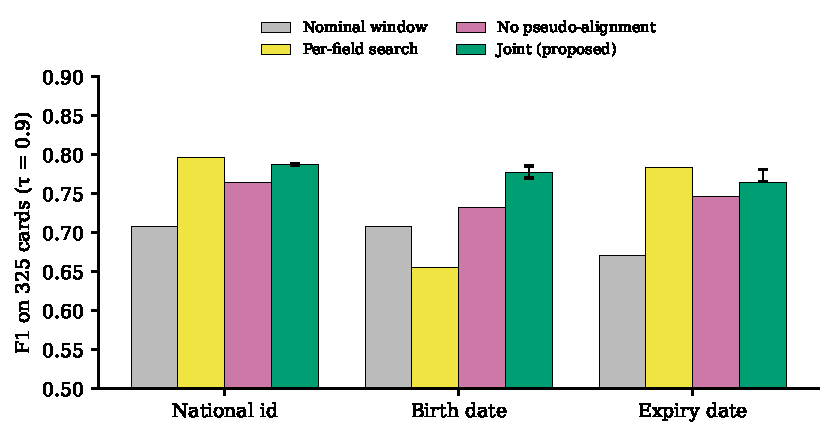
\includegraphics[width=0.85\textwidth]{figures/ablation.pdf}
\caption{Ablation $\Fone$ per field. The error bars on the joint variant are the standard deviation over three seeds.}\label{fig:abl}
\end{figure}

\subsection{Confidence as a decision signal}
Fig.~\ref{fig:conf} (left) shows precision of accepted values against coverage as $\tau$ varies, and (right) the confidence distribution of correct and incorrect readings. The AUC of the confidence for correctness is 0.997, 0.994 and 0.997 for the three fields, and the ECE over well-formed readings is 0.016 (Fig.~\ref{fig:rel}). Calibration is good on this test set, but $\tau$ was not validated on a separate split.
\begin{figure}[t]
\centering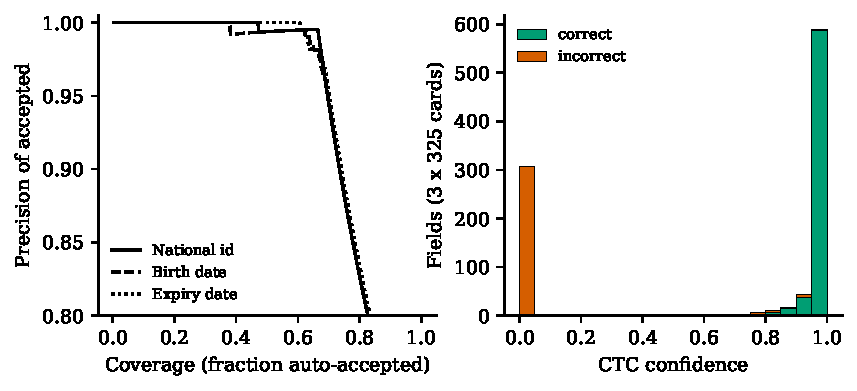
\includegraphics[width=\textwidth]{figures/confidence.pdf}
\caption{Left: precision--coverage curves. Right: CTC confidence of correct and incorrect readings (325 cards, three fields).}\label{fig:conf}
\end{figure}
\begin{figure}[t]
\centering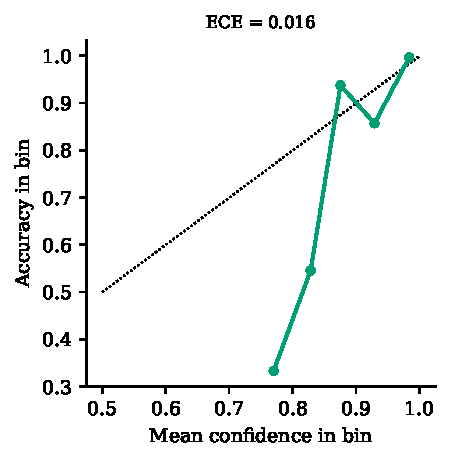
\includegraphics[width=0.4\textwidth]{figures/reliability.pdf}
\caption{Reliability diagram of the CTC confidence.}\label{fig:rel}
\end{figure}

\subsection{Negative results}
Warping to a median face box worsened identifier accuracy from 41.8\% to 36.8\%. A shear search on the digit line broke the slanted date separator. Adding 144 late-arriving photographs (1{,}856 to 2{,}000) gave about one point.

\section{Limitations}
The data are fictitious, single-design and single-source; one train/test split was used and no $k$-fold; $\tau$ was fixed rather than validated; about 45\% of photographs yield no confident reading (46 of 400 are rejected before OCR); names are read poorly (about 25\%) and always flagged for review; baselines are limited to engines runnable on CPU without network access (TrOCR and PaddleOCR were not evaluated); and no real identity documents were used. The conclusions concern relative gains on this benchmark and do not establish production accuracy.

\section{Conclusion}
Verifying alignment against known labels and registering by recognition lift a small CPU-only CRNN from 0.49 to 0.71 macro $\Fone$ on hand-held photographs of a synthetic ID-card dataset, with calibrated confidence for review routing. Validation on a second benchmark and on consented real documents is the next step.

\paragraph{Reproducibility.} Code, layouts and the figure/table generator are in the project repository; the dataset and trained weights are not redistributed because the licence is unconfirmed.

\bibliographystyle{unsrtnat}
\bibliography{references}
\end{document}
